% -*- TeX-master: "master.tex" -*-
\section{Identical Particles}
\subsection{Two-Particle Systems}
Multi-particle systems must also obey the Schrodinger equation, but for each individual particle. So the Hamiltonian is:
\begin{align*}
  \hat{H}=-\dfrac{\hbar^2}{2m_1}\laplacian_1-\dfrac{\hbar^2}{2m_2}\laplacian_2
  +V(\vb{r}_1,\vb{r}_2,t)
\end{align*}
The new normalization condition is:
\begin{align*}
  \int\abs{\Psi(\vb{r}_1,\vb{r}_2,t)}^2\dd[3]{\vb{r}_1}\dd[3]{\vb{r}_2}
\end{align*}
We are integrating in this case over the entire volume with respect to the first and second particles. We can introduce the same time dependence assuming a potential which is not time dependent:
\begin{align*}
  \Psi(\vb{r}_1,\vb{r}_2,t)=\psi(\vb{r}_1,\vb{r}_2)\exp{-iEt/\hbar}
\end{align*}
Now the spatial wavefunction is left with:
\begin{align*}
  -\dfrac{\hbar^2}{2m_1}\laplacian_1\psi-\dfrac{\hbar^2}{2m_2}\laplacian_2\psi+V\psi=E\psi
\end{align*}
Suppose these particles do not interact with one another, this means that the potential can be written strictly as:
\begin{align*}
  V(\vb{r}_1,\vb{r}_2)=V_1(\vb{r}_1)+V_2(\vb{r}_2)
\end{align*}
We can separate variables by setting:
\begin{align*}
  \psi(\vb{r}_1,\vb{r}_2)=\psi_a(\vb{r}_1)\psi_b(\vb{r}_2)
\end{align*}
We can introduce constants $E_a$ and $E_b$ such that $E=E_a+E_b$, and get a separate Schrodinger equation for each particle:
\begin{align*}
  -\dfrac{\hbar^2}{2m_1}\laplacian_1\psi_a+V_1(\vb{r}_1)&=E_a\psi_a\\
  -\dfrac{\hbar^2}{2m_2}\laplacian_2\psi_b+V_2(\vb{r}_2)&=E_b\psi_b
\end{align*}
The full wavefunction is:
\begin{align*}
  \Psi(\vb{r}_1,\vb{r}_2,t)&=\psi_a(\vb{r}_1)\psi_b(\vb{r}_2)\exp{-i(E_a+E_b)t/\hbar}\\
  &=\qty(\psi_a(\vb{r}_1)\exp{-iE_at/\hbar})\qty(\psi_b(\vb{r}_2)\exp{-iE_bt/\hbar})\\
  &=\Psi_a(\vb{r}_1,t)\Psi_b(\vb{r}_2,t)
\end{align*}
Another case to consider is the central potential, such that the potential is:
\begin{align*}
  V(\vb{r}_1,\vb{r}_2)=V(\abs{\vb{r}_1-\vb{r}_2})
\end{align*}
An example of this is the hydrogen atom potential. However, in general, there may be external forces and ineraction forces, such as the two electrons in a helium atom, there is the attraction to the proton from both charges, then they mutually attract one another. 
\subsubsection{Bosons and Fermions}
Suppose we have two non-interacting particles, one in the state $\psi_a$, and the other in $\psi_b$, so the total wavefunction of the system:
\begin{align*}
  \psi(\vb{r}_1,\vb{r}_2)=\psi_a(\vb{r}_1)\psi_b(\vb{r}_2)
\end{align*}
This however, assumes that the particles are distinguishable, that is we can tell which particle is $1$ and which is $2$. In reality, all electrons are indistinguishable. There is really no such thing as this or that electron, they are all essentially identical. To remedy this, we introduce either an added or subtracted other term, a linear combination, since this is also a valid state:
\begin{align*}
  \psi_\pm(\vb{r}_1,\vb{r}_2)=\dfrac{1}{\sqrt{2}}
  \qty(\psi_a(\vb{r}_1)\psi_b(\vb{r}_2)\pm\psi_a(\vb{r}_2)\psi_b(\vb{r}_1))
\end{align*}
This theory gives two types of particles, bosons, where the state is symmetric under exchange of the particles, and fermions, where the state is anti-symmetric under exchange. It turns out that particles with integer spin are bosons, and particles with half integer spin are fermions. From the anti-symmetry of the fermion state we get the famous Pauli exclusion principle, which states that two fermions cannot occupy the same state, as if they did:
\begin{align*}
  \psi_-(\vb{r}_1,\vb{r}_2)=\dfrac{1}{\sqrt{2}}\qty
      [\psi_a(\vb{r}_1)\psi_b(\vb{r}_2)-\psi_a(\vb{r}_2)\psi_b(\vb{r}_1)]
\end{align*}
\subsubsection{Exchange Forces}
Consider a $1-D$ example, we have a particle in one state $\psi_a(x)$ and another in a state $\psi_b(x)$, the distinguishable case has the total combined wavefunction as:
\begin{align*}
  \psi(x_1,x_2)=\psi_a(x_1)\psi_b(x_2)
\end{align*}
Identical bosons produce the following:
\begin{align*}
  \psi_+(x_1,x_2)=\dfrac{1}{\sqrt{2}}\qty(\psi_a(x_1)\psi_b(x_2)+\psi_b(x_1)\psi_a(x_2))
\end{align*}
And last but not least identical fermions have:
\begin{align*}
  \psi_-(x_1,x_2)=\dfrac{1}{\sqrt{2}}\qty(\psi_a(x_1)\psi_b(x_2)-\psi_b(x_1)\psi_a(x_2))
\end{align*}
Lets find the average value of the square separation distance:
\begin{align*}
  \ev{(x_1-x_2)^2}=\ev{x_1^2}+\ev{x_2^2}-2\ev{x_1x_2}
\end{align*}
For identical particles, we can exactly separate the integrals:
\begin{align*}
  \ev{x_1^2}=\int x_1^2\abs{\psi_a(x_1)}^2\dd{x_1}\int\abs{\psi_b(x_2)}^2\dd{x_2}
\end{align*}
The second integral is just the normalization condition, and the second is the expectation value of $x^2$ in $\psi_a$:
\begin{align*}
  \ev{x_1^2}=\ev{x^2}_a
\end{align*}
A similar integral appears in the $x_2^2$:
\begin{align*}
  \ev{x_1^2}=\int\abs{\psi_a(x_1)}^2\dd{x_1}\int x^2\abs{\psi_b(x_2)}^2\dd{x_2}=\ev{x^2}_b
\end{align*}
The last one has:
\begin{align*}
  \ev{x_1x_2}=\int x_1\abs{\psi_a(x_1)}^2\dd{x_1}\int x_2\abs{\psi_b(x_2)}^2\dd{x_2}=
  \ev{x}_a\ev{x}_b
\end{align*}
The overall expectation value will be:
\begin{align*}
  \ev{(x_1-x_2)^2}_d=\ev{x^2}_a+\ev{x^2}_b-2\ev{x}_a\ev{x}_b
\end{align*}
The situation is a bit different for identical particles:
\begin{align*}
  \ev{x_1^2}=&\dfrac{1}{2}
  \left[\int x_1^2\abs{\psi_a(x_1)}^2\dd{x_1}\int\abs{\psi_b(x_2)}^2\dd{x_2}\right.\\
    &+\int x_1^2\abs{\psi_b(x_1)}^2\dd{x_1}\int\abs{\psi_a(x_2)}^2\dd{x_2}\\
    &\pm\int x_1^2\psi_a(x_1)^*\psi_b(x_1)\dd{x_1}\int\psi_b(x_2)^*\psi_a(x_2)\dd{x_2}\\
    &\left.\pm\int x_1^2\psi_b(x_1)^*\psi_a(x_1)\dd{x_1}\int\psi_a(x_2)^*\psi_b(x_2)
    \dd{x_2} \right]\\
  &=\dfrac{1}{2}\qty[\ev{x^2}_a+\ev{x^2}_b\pm0\pm0]
  =\dfrac{1}{2}\qty[\ev{x^2}_a+\ev{x^2}_b]
\end{align*}
We can similarly find:
\begin{align*}
  \ev{x_2^2}=\dfrac{1}{2}\qty[\ev{x^2}_a+\ev{x^2}_b]
\end{align*}
As for the product, we have:
\begin{align*}
  \ev{x_1x_2}=&\dfrac{1}{2}
  \left[\int x_1\abs{\psi_a(x_1)}^2\dd{x_1}\int x_2\abs{\psi_b(x_2)}^2\dd{x_2}\right.\\
    &+\int x_1\abs{\psi_b(x_1)}^2\dd{x_1}\int x_2\abs{\psi_a(x_2)}^2\dd{x_2}\\
    &\pm\int x_1\psi_a(x_1)^*\psi_b(x_1)\dd{x_1}\int x_2\psi_b(x_2)^*\psi_a(x_2)\dd{x_2}\\
    &\left.\pm\int x_1\psi_b(x_1)^*\psi_a(x_1)\dd{x_1}
    \int x_2\psi_a(x_2)^*\psi_b(x_2)\dd{x_2}\right]\\
  &=\dfrac{1}{2}\qty[\ev{x}_a\ev{x}_b+\ev{x}_b\ev{x}_a
    \pm\ev{x}_{ab}\ev{x}_{ba}\pm\ev{x}_{ba}\ev{x}_{ab}]\\
  &=\ev{x}_a\ev{x}_b\pm\abs{\ev{x}_{ab}}^2
\end{align*}
Hence the average squared distance is:
\begin{align*}
  \ev{(x_1-x_2)^2}_\pm=\ev{x^2}_a+\ev{x^2}_b-2\ev{x}_a\ev{x}_b\mp2\abs{\ev{x}_{ab}}^2
\end{align*}
However, we can see some similarities with the previous result, we can see that:
\begin{align*}
  \ev{(\Delta x)^2}_\pm=\ev{(\Delta x)^2}_d\mp2\abs{\ev{x}_{ab}}^2
\end{align*}
\subsubsection{Spin}
The complete state of say, an electron, includes not only its spatial state, but also its spin state:
\begin{align*}
  \psi=\psi(\vb{r})\chi
\end{align*}
The two particle state contains:
\begin{align*}
  \psi(\vb{r}_1,\vb{r}_1)\chi(1,2)
\end{align*}
This entire wavefunction needs to be anti-symmetric under exchange:
\begin{align*}
  \psi(\vb{r}_1,\vb{r}_1)\chi(1,2)=-\psi(\vb{r}_2,\vb{r}_1)\chi(2,1)
\end{align*}
Something important to note is that this means only one of the spin and spatial states must be anti-symmetric.
\subsubsection{Generalized Symmetrization Principle}
Define the exchange operator $\hat{P}$:
\begin{align*}
  \hat{P}\ket{1,2}=\ket{2,1}
\end{align*}
Clearly $\hat{P}^2=1$, the identity operator, and because of this, we get eigenvalues of $\pm1$. Clearly this operator commutes with the Hamiltonian. This means that the system will stay anti-symmetric/symmetric. The eigenvalue corresponding to symmetry is $1$ and anti-symmetry is $-1$. In general if you have $n$ identical particles, swapping any two of them should be (anti)symmetric. 
\subsection{Atoms}
The general Hamiltonian of an atom with atomic number $Z$ is:
\begin{align*}
  \hat{H}=\sum_{j=1}^{Z}\qty[\dfrac{-\hbar^2}{2m}\laplacian_j-
    \qty(\dfrac{1}{4\pi\veps_0})\dfrac{Ze^2}{r_j}]
  +\dfrac{1}{2}\qty(\dfrac{1}{4\pi\veps_0})\sum_{j\neq k}^Z
  \dfrac{e^2}{\abs{\vb{r}_j-\vb{r}_k}}
\end{align*}
However, we cannot solve the Schrodinger equation with the above Hamiltonian exactly. For a simpler atom, we can do the Helium atom:
\begin{align*}
  \hat{H}=
  \qty[\dfrac{-\hbar^2}{2m}\laplacian_1-\qty(\dfrac{1}{4\pi\veps_0})\dfrac{Ze^2}{r_1}]
  +\qty[\dfrac{-\hbar^2}{2m}\laplacian_2-\qty(\dfrac{1}{4\pi\veps_0})\dfrac{Ze^2}{r_2}]
  +\dfrac{1}{4\pi\veps_0}\dfrac{e^2}{\abs{\vb{r}_1-\vb{r}_2}}
\end{align*}
For our sake, we will ignore the attraction term, giving the full wavefunction of:
\begin{align*}
  \psi(\vb{r}_1,\vb{r}_2)=\psi_{n\ell m}(\vb{r}_1)\psi_{n'\ell'm'}
\end{align*}
Its ground state would be a symmetric state with both having $100$ as their quantum numbers. This means that the spin state of the electrons must be anti-symmetric. This means that spin states must be oppositely aligned, so it is a singlet state. The excited states of helium consist of one electron in the hydrogenic ground state, and the other in an excited state. The helium with an anti-symmetric spin state will be called parahelium, orthohelium, the other type, requires a symmetric spin state.
\subsubsection{Hund's Rules and Spectroscopic Notation}
Hund's first rule says that the state with the lowest energy will have the highest total spin. Hund's second rule says that the state with highest angular momentum should have the lowest energy. Hund's third rule says that if a sub-shell is no more than half filled, then the lowest energy level has $J=\abs{L-S}$, if it is more than half full, then $J=L+S$. Spectroscopic notation takes the form of:
\begin{align*}
  ^{2S+1}L_{J}
\end{align*}
Which can be determined by Hund's rules. Use the following steps:
\begin{enumerate}
\item Write out your best guess for the electron configuration.
\item Now we want to maximize $S$ (assuming we couple $L$ and $S$, so we write out the outermost shell, it can either be $s$, $p$, $d$, or maybe $f$. Use the following pictures as a guide for how many steps to put:
  \begin{figure}[H]
    \centering
    \begin{tikzpicture}
      % s
      \draw (-0.25,0) circle (0) node {s};
      \draw (0,0) -- node[below] {0} (1,0);
      % p
      \draw (2-0.25,0) circle (0) node {p};
      \draw (2, 0) -- node[below] { 0} (3, 0);
      \draw (2, 1) -- node[below] {-1} (3, 1);
      \draw (2,-1) -- node[below] { 1} (3,-1);
      % d
      \draw (4-0.25,0) circle (0) node {d};
      \draw (4, 2) -- node[below] {-2} (5, 2);
      \draw (4, 1) -- node[below] {-1} (5, 1);
      \draw (4, 0) -- node[below] { 0} (5, 0);
      \draw (4,-1) -- node[below] { 1} (5,-1);
      \draw (4,-2) -- node[below] { 2} (5,-2);
    \end{tikzpicture}
    \caption{Possible $m$ values for $s,p,d$}
  \end{figure}
  Now, depending on how many electrons are in the outer shell, place as many up arrows in as many open spots as possible, without placing any down arrows, for example, the Fe atom ground state has $6$ electrons in its valence shell, so this diagram will give the following:
  \begin{figure}[H]
    \centering
    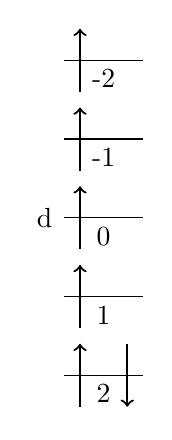
\begin{tikzpicture}
      % d
      \draw (0-0.25,0) circle (0) node {d};
      \draw (0, 2) -- node[below] {-2} (1, 2);
      \draw (0, 1) -- node[below] {-1} (1, 1);
      \draw (0, 0) -- node[below] { 0} (1, 0);
      \draw (0,-1) -- node[below] { 1} (1,-1);
      \draw (0,-2) -- node[below] { 2} (1,-2);
      \draw[->,thick] (0.2, 2-0.4) -- (0.2, 2+0.4);
      \draw[->,thick] (0.2, 1-0.4) -- (0.2, 1+0.4);
      \draw[->,thick] (0.2, 0-0.4) -- (0.2, 0+0.4);
      \draw[->,thick] (0.2,-1-0.4) -- (0.2,-1+0.4);
      \draw[->,thick] (0.2,-2-0.4) -- (0.2,-2+0.4);
      \draw[<-,thick] (0.8,-2-0.4) -- (0.8,-2+0.4);
    \end{tikzpicture}
    \caption{Ground State of Fe}
  \end{figure}
\item Find $L$ by adding up all of the values on the sides for every electron that is present, in the example above, we would have $L=2+2+1+0-1-2=2$. 
\item The term symbol changes depending on $L$, the most common are $S,P,D,F$ for $L=0,1,2,3$ respectively
\item Find $S$ by adding $1/2$ for every up arrow, and adding $-1/2$ for every down arrow. Multiply it by two and add 1 to get the upper left symbol
\item If the shell is half full or more than half full, get the lower right symbol by adding $L$ and $S$, it is less than half full, take the absolute value of their difference. 
\end{enumerate}
\subsection{Solids}
In solids, the valence electrons are free to move, there are two models we will look at, the electron gas and the Bloch model
\subsubsection{The Free Electron Gas}
Suppose we have a rectangular solid, with dimensions $l_x$, $l_y$ and $l_z$, and an electron inside experiences no forces at all except at the walls:
\begin{align*}
  V(x,y,z)=
  \begin{cases}
    0 & 0<x<l_x,0<y<l_y,0<z<l_z\\
    \infty & \text{otherwise}
  \end{cases}
\end{align*}
The Schrodinger equation gives:
\begin{align*}
  -\dfrac{\hbar^2}{2m}\laplacian{\psi}=E\psi
\end{align*}
In Cartesian coordinates we get:
\begin{align*}
  -\dfrac{\hbar^2}{2m}\dv[2]{X}{x}=E_xX\qquad
  -\dfrac{\hbar^2}{2m}\dv[2]{Y}{y}=E_yY\qquad
  -\dfrac{\hbar^2}{2m}\dv[2]{Z}{z}=E_zZ
\end{align*}
Where the total energy is the sum $E_x+E_y+E_z$, Using usual coefficient substitution we have:
\begin{align*}
  k_x\equiv\dfrac{\sqrt{2mE_x}}{\hbar}\qquad
  k_y\equiv\dfrac{\sqrt{2mE_y}}{\hbar}\qquad
  k_z\equiv\dfrac{\sqrt{2mE_z}}{\hbar}
\end{align*}
The first boundary conditions give:
\begin{align*}
  X(x)=A_x\sin(k_xx)\qquad Y(y)=A_y\sin(k_yy)\qquad Z(z)=A_z\sin(k_zz)
\end{align*}
And we get restrictions on the $k$s from the other condition:
\begin{align*}
  k_xl_x=n_x\pi\qquad k_yl_y=n_y\pi\qquad k_zl_z=n_z\pi
\end{align*}
And each of the $n_i$ is a positive integer. Going through the regular infinite square well normalization gives:
\begin{align*}
  \psi_{n_xn_yn_z}=\sqrt{\dfrac{8}{l_xl_yl_z}}
  \sin(\dfrac{n_x\pi}{l_x}x)\sin(\dfrac{n_y\pi}{l_y}y)\sin(\dfrac{n_z\pi}{l_z}z)
\end{align*}
And the energies are:
\begin{align*}
  E_{n_xn_yn_z}=\dfrac{\hbar^2\pi^2}{2m}
  \qty(\dfrac{n_x^2}{l_x^2}+\dfrac{n_y^2}{l_y^2}+\dfrac{n_z^2}{l_z^2})=
  \dfrac{\hbar^2k^2}{2m}
\end{align*}
We now shift to a space where the axes are given by the three $k$ variables, and lines are drawn at $\pi/l_i$. This means each block occupies a space with the volume:
\begin{align*}
  \dfrac{\pi^3}{l_xl_yl_z}=\dfrac{\pi^3}{V}
\end{align*}
But this is not a volume in the traditional sense, it a volume in $k$-space. The solid contains $N$ atoms with $d$ free electrons per atom. If the electrons were distinguishable, or bosons, they would all be in the $\psi_{111}$ state, but alas they are not, due to the Pauli exclusion principle they cannot all occupy $\psi_{111}$ together. These electrons will fill out an octant of a sphere in $k$-space, whose radius is some Fermi wavenumber $k_F$. Since each pair of electrons effectively fills an chunk in $k$-space, we have:
\begin{align*}
  \dfrac{1}{8}\qty(\dfrac{4}{3}\pi k_F^3)=\dfrac{Nd}{2}\qty(\dfrac{\pi^3}{V})
\end{align*}
Solving for $k_F$ results in:
\begin{align*}
  k_F^3=\dfrac{3Nd\pi^2}{V}=3\rho\pi^2
\end{align*}
Where $\rho$ is the free electron density. This Fermi wavenumber defines a Fermi energy given by:
\begin{align*}
  E_F=\dfrac{\hbar^2}{2m}\qty(3\rho\pi^2)^{3/2}
\end{align*}
The total energy of the electron gas can be calculated by finding the volume of a shell with thickness $\dd{k}$:
\begin{align*}
  \dd{V}=\dfrac{1}{8}\qty(4\pi k^2)\dd{k}
\end{align*}
The number of states in the shell is:
\begin{align*}
  \dfrac{2\qty((1/2)\pi k^2\dd{k})}{\pi^3/V}=\dfrac{V}{\pi^2}k^2\dd{k}
\end{align*}
So the differential energy is:
\begin{align*}
  \dd{E}=\dfrac{\hbar^2}{2m}\dfrac{V}{\pi^2}k^2\dd{k}=\dfrac{\hbar^2V}{2\pi^2m}k^4\dd{k}
\end{align*}
So the total energy of filled states is:
\begin{align*}
  E_{tot}=\dfrac{\hbar^2V}{2\pi^2m}\int_0^{k_F}k^4\dd{k}=\dfrac{\hbar^2k_F^5V}{10\pi^2m}=
  \dfrac{\hbar^2(3\pi^2Nd)^{5/3}}{10\pi^2m}V^{-2/3}
\end{align*}
\subsubsection{Band Structure}
We start this section by defining a periodic potential, such that:
\begin{align*}
  V(x+a)=V(x)
\end{align*}
Bloch's theorem says that the such potentials satisfy the Schrodinger equation with an additional boundary condition:
\begin{align*}
  \psi(x+a)=\exp{iqa}\psi(x)
\end{align*}
The constant $q$ is independent of position, it may however depend on other factors. It is important to note that this additional phase does not change the normalization:
\begin{align*}
  \abs{\psi(x+a)}^2=\abs{\psi(x)}^2
\end{align*}
Now, no real solid goes on forever, so we can just wrap the $x$ axis around after some point $N$:
\begin{align*}
  \psi(x+Na)=\psi(x)
\end{align*}
So we get that:
\begin{align*}
  \exp{iNqa}\psi(x)=\psi(x)
\end{align*}
So we have that:
\begin{align*}
  \exp{iNqa}=1\implies Nqa=2\pi n
\end{align*}
And the values of $q$ are:
\begin{align*}
  q=\dfrac{2\pi n}{Na}
\end{align*}
Where $n =0,\pm1,\pm2...$. One potential we can consider is the Dirac comb:
\begin{align*}
  V(x)=\alpha\sum_{j=0}^{N-1}\delta(x-ja)
\end{align*}
We solve the Schrodinger equation in the region between delta functions:
\begin{align*}
  \dv[2]{\psi}{x}=-\dfrac{2mE}{\hbar^2}\psi=-k^2\psi
\end{align*}
Which has the general solution of:
\begin{align*}
  \psi(x)=A\sin(kx)+B\cos(kx)
\end{align*}
Invoking Bloch's theorem, the wavefunction immediately left of the origin is:
\begin{align*}
  \psi(x)=\exp{-iqa}\qty(A\sin(k(x+a))+B\cos(k(x+a)))
\end{align*}
The wavefunction must be continuous at $x=0$, so we get:
\begin{align*}
  B=\exp{-iqa}\qty[A\sin(ka)+B\cos(ka)]
\end{align*}
The derivative inherits the discontinuity as well, so we get from previous quantities:
\begin{align*}
  kA-\exp{-iqa}k\qty(A\cos(ka)-B\sin(ka))=\dfrac{2m\alpha}{\hbar^2}B
\end{align*}
We can solve for $A\sin(ka)$:
\begin{align*}
  A\sin(ka)=\qty[\exp{iqa}-\cos(ka)]B
\end{align*}
Using the other equation, we can find that:
\begin{align*}
  \qty[\exp{iqa}-\cos(ka)]\qty[1-\exp{-iqa}\cos(ka)]+\exp{-iqa}\sin^2(ka)=
  \dfrac{2m\alpha}{\hbar^2k}\sin(ka)
\end{align*}
This can simplify to:
\begin{align*}
  \cos(qa)=\cos(ka)+\dfrac{m\alpha}{\hbar^2k}\sin(ka)
\end{align*}
This is a transcendental equation, we define $z\equiv ka$ and $\beta\equiv m\alpha a/\hbar^2$. Giving the right side as:
\begin{align*}
  f(z)\equiv\cos(z)+\beta\dfrac{\sin(z)}{z}
\end{align*}
Where we can find intersections with $\pm1$ since $\cos(qa)$ is going to be one of those. 
